
\chapter{Using the MGX application}
\label{using}

\section{Basic concepts}

\subsection{Metadata}

In addition to the sequence data, MGX requires a user to provide additional information
about a dataset, e.g. further details about the investigated habitat as well as sampling
and sequencing procedures. Metadata in the MGX platform is organized in a hierarchical
manner describing

\begin{itemize}
  \item the geographical location of a habitat,
  \item the sample taken from a habitat,
  \item the DNA extraction procedure,
  \item sequencing technology and protocol.
\end{itemize}

\subsection{Read-based analysis: Attributes and attribute types}

\section{Obtaining a MGX project}

Currently, there is no way to automatically create new MGX projects. If you would like to
analyse your data using MGX, send a mail to the MGX team, which can be contacted at 
\href{mailto:mgx@CeBiTec.Uni-Bielefeld.DE}{mgx@CeBiTec.Uni-Bielefeld.DE}. MGX projects
and users are managed by the General Project Management System (GPMS) developed at CeBiTec,
which provides Single Sign-On (SSO) for all applications provided by CeBiTec's Computational
Genomics group.

To apply for a new project, include information about

\begin{itemize}
  \item suggested \textit{project name}, e.g. MGX\_AcidMine
  \item a short \textit{one-line description} of your project (''Acid Mine Drainage metagenome'')
  \item a \textit{contact address} of a single person responsible for the project (PI or group leader)
  \item a \textit{list of all users} that should be granted project access, including
    \begin{itemize}
      \item Full name and email address for users not yet registered in the GPMS system, GPMS username otherwise
      \item desired access level
    \end{itemize}
\end{itemize}

MGX offers different access levels (roles), which are assigned individually for each
project: \\

\begin{itemize}
  \item{\textbf{Admins} are equal to Users (see below), but can grant access to additional users.}
  \item \textbf{Users} have full access to a MGX project and are able to define new or modify
present datasets, import new sequences and execute analysis jobs. They are also able to
delete all data associated with a project.
  \item \textbf{Guests} are provided read-only access to a project, i.e. they are able to access
all information already present, view analysis results and export data; however, they are
unable to perform new analysis or delete data from the project.
\end{itemize}

As new users can always be added to an existing MGX project, all registered users are required
to carefully protect their login credentials and not to share them with any third party.

\section{Connecting to a MGX server}

After installation, the MGX application is already preconfigured to connect to the 
MGX server instance hosted at CeBiTec, Bielefeld University. In case a different MGX server
should be used, the default server can be changed choosing Tools $->$ Options from the menu
and navigating to the MGX server tab (\ref{config-site}). While the site name can be freely
chosen by the user, the server URL has to be entered as provided by the server administrators.

\begin{figure}[ht]
\centering
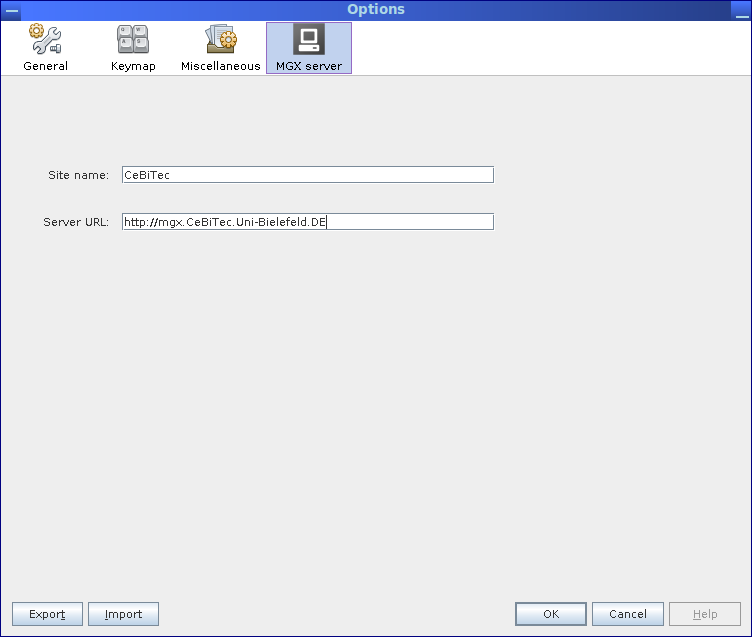
\includegraphics[width=.8\textwidth]{img/configure-site}
\caption[Server configuration:]{A different server instance can be configured in the MGX 
server tab available from the Tools -> Options menu.}
\label{config-site}
\end{figure}


\begin{figure}[ht]
\centering
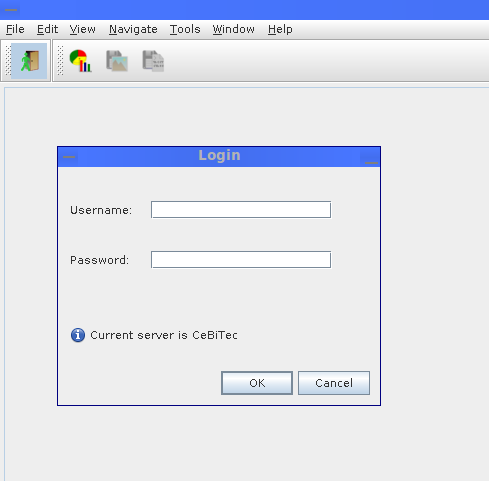
\includegraphics[width=.8\textwidth]{img/login-screen}
\caption[Login screen:]{The login screen also reflects the name of the configured server.}
\label{login-screen}
\end{figure}

All communication between the MGX user interface and the MGX server is encrypted using
the standardized SSL (Secure Sockets Layer) protocol, ensuring confidentiality of 
unpublished data and protecting the integrity of login credentials.

\section{Browsing and exploring MGX projects}

After successfully logging in, a new window is automatically opened. The MGX Explorer window
lists all available projects a user is allowed to access, including both public as well as
private projects. Projects are easily opened or closed by simply expanding the corresponding
nodes in the project explorer window (\ref{structure}).\\

\begin{figure}[ht]
\centering
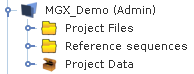
\includegraphics[width=.4\textwidth]{img/projstructure}
\caption[Project structure:]{Divided into three different parts, a MGX projects offers
(from top to bottom) dedicated storage for files to be used by analysis pipelines, 
managed reference sequences (including annotation data, if available) and general
project data containing metadata as well as sequence datasets.}
\label{structure}
\end{figure}


Each project contains metagenome datasets as well as structured storage, where user-provided
databases can be uploaded to be used in custom analysis (\ref{custom}).

TODO: Screenshot explorer

\section{Creating a new habitat}

New habitats are defined choosing ''Add habitat'' from the context menu 
\section{Creating a new sample}
\section{Creating a new DNA extract}
\section{Importing sequence data}
\section{Defining and executing analysis jobs}
\subsection{Selecting a tool}
\subsection{Setting parameters}
\subsection{Monitoring job progress}
\section{Visualization of results}
\subsection{Choosing data sets}
\subsection{Choosing a visualisation type}
\subsection{Exporting sequences}
\section{Search}


